%Documento di proprietà di Vito Stefano Birardi™
%Qui sono presenti i package più comuni che usi, ricorda di usare solo quelli che ti servono 

%Variabili comuni
\newcommand{\Titolo}{Progetto Quality Treshold - Documentazione}
\newcommand{\Data}{19/06/2025}
\newcommand{\Materia}{}

%Comandi troppo lunghi da scrivere possono essere ri-operazionalizzati qui

\newcommand{\image}[3]{
    \begin{figure}[h!]
    \centering
    \includegraphics[width = \textwidth]{#1}
    \caption{#2}
    \label{#3}
\end{figure}}

%Package per la formattazione del foglio

\documentclass[a4paper]{article}
\usepackage{amsmath}
\usepackage{amssymb}

%Package per la lingua dei capitoli

\usepackage[italian]{babel}

%Package per intestazione e pié di pagina

\usepackage{fancyvrb}
\usepackage{fancyhdr, lastpage}

%Package aggiuntivi 

\usepackage{cancel}
\usepackage{etoolbox}
\usepackage{xcolor}
\usepackage{subfig}
\usepackage{tikz, lmodern}
\usepackage[T1]{fontenc}
\usepackage[most]{tcolorbox}
\usepackage{graphicx}
\usepackage{hyperref}
\usepackage{parskip}
\usepackage{multicol}
\pagestyle{fancy}

%Formattazione hyperlinks

\hypersetup{
    colorlinks=true,
    linkcolor=blue,
    filecolor=magenta, 
    urlcolor=blue,
    pdfpagemode=FullScreen
}

%Formattazione di intestazione e pié di pagina

\lhead{\Data}
\rhead{Vito Stefano Birardi}
\lfoot{\Materia}
\rfoot{Pagina \thepage\ di \hyperlink{toc}{\pageref*{LastPage}}}
\renewcommand{\footrulewidth}{0.5pt}
\fancyfoot[C]{}
\patchcmd{\chapter}{\thispagestyle{plain}}{\thispagestyle{fancy}}{}

%Preambolo per prima pagina

\title{\Titolo}
\author{
    A cura di: 
    Vito Stefano Birardi
}
\date{\Data}

%Inizio documento vero e proprio


\begin{document}
\maketitle
\newpage
\hypertarget{toc}{\tableofcontents}
\newpage
\section{Introduzione}


Il progetto in questione utilizza l'algoritmo \textbf{Quality Threshold (QT)} per l'analisi dei dati. Tali dati possono essere estratti da un file o dalle tabelle di un database MySQL.

\section{Cos'è l'Algoritmo Quality Threshold}

L'algoritmo Quality Threshold è un algoritmo di \textbf{clustering} deterministico che appartiene alla famiglia degli algoritmi di raggruppamento gerarchico. A differenza degli algoritmi di partizionamento tradizionali, il QT non richiede di specificare a priori il numero di cluster da creare, ma si basa su un parametro di soglia di qualità (\textit{threshold}) che definisce il raggio massimo consentito per ogni cluster.

\section{Principio di Funzionamento}

L'algoritmo si basa sulla \textbf{minimizzazione della distanza} tra i punti dati e il centroide del cluster di appartenenza. Il processo di clustering avviene attraverso i seguenti passaggi:

\begin{enumerate}
\item \textbf{Selezione del punto candidato}: Per ogni punto del dataset, viene valutata la possibilità di creare un nuovo cluster
\item \textbf{Formazione del cluster}: Vengono raggruppati tutti i punti che si trovano entro il raggio di soglia specificato
\item \textbf{Selezione del cluster ottimale}: Viene scelto il cluster che contiene il maggior numero di punti
\item \textbf{Iterazione}: Il processo si ripete sui punti rimanenti fino a quando tutti i punti sono stati assegnati a un cluster
\end{enumerate}

\section{Caratteristiche Distintive}

L'algoritmo Quality Threshold presenta diverse caratteristiche che lo distinguono da altri approcci di clustering:

\subsection{Vantaggi}

\begin{itemize}
\item \textbf{Determinismo}: L'algoritmo restituisce sempre lo stesso risultato quando viene eseguito ripetutamente sullo stesso dataset, a differenza di algoritmi come il \textit{k-means} che possono produrre risultati diversi a seconda dell'inizializzazione casuale
\item \textbf{Numero di cluster automatico}: Non richiede di specificare il numero di cluster da creare, ma solo il raggio massimo (\textit{threshold}), rendendo l'algoritmo più flessibile per dataset con strutture sconosciute
\item \textbf{Robustezza al rumore}: È stato progettato per gestire efficacemente dati rumorosi e con distribuzioni non lineari
\item \textbf{Approccio gerarchico}: Utilizza una strategia gerarchica per la creazione dei cluster, garantendo una maggiore stabilità dei risultati
\end{itemize}

\subsection{Svantaggi}

\begin{itemize}
\item \textbf{Complessità computazionale}: Richiede una potenza di calcolo maggiore rispetto ad algoritmi di partizionamento come il \textit{k-means}, con una complessità temporale che può essere significativamente elevata per dataset di grandi dimensioni
\item \textbf{Sensibilità al parametro threshold}: La scelta del raggio di soglia influenza notevolmente la qualità del clustering ottenuto
\end{itemize}

\section{Ambiti di Applicazione}

L'algoritmo Quality Threshold è particolarmente adatto per contesti in cui:

\begin{itemize}
\item I dati presentano rumore significativo
\item La distribuzione dei dati è non lineare o presenta forme complesse
\item Non si conosce a priori il numero ottimale di cluster
\item È richiesta riproducibilità dei risultati
\item La qualità del clustering è più importante dell'efficienza computazionale
\end{itemize}
\section{Guida all'installazione}

Prima di essere in grado di eseguire il programma, è necessario eseguire il file \texttt{risorse.bat} contenuto nella cartella Risorse. 


Una volta eseguito il file, si aprirà una pagina di Powershell e seguirà un download.

\begin{figure}[h!]
    \centering
    
\includegraphics[width= 0.5\textwidth]{images/nuova docs.png}
    \caption{Schermatta di download}
\end{figure}

Al termine del download del file compresso delle risorse, verranno estratti i file necessari per l'esecuzione del programma.



Per il progetto in questione è necessario installare il Java Developer Kit (JDK) nella versione 22.0.1 e il software di gestione del database MySQL nella sua versione 8.0.39. 

La prima scheda di installazione che apparirà è quella del JDK. 

Verrà chiesto se si vuole eseguire l'installazione del JDK tramite permessi di amministratore, cliccare su \underline{Sì}.

\subsection{Installazione JDK}

Una volta confermata l'esecuzione come amministratore, si procederà all'installazione del JDK.

\begin{figure}[h!]
    \centering
    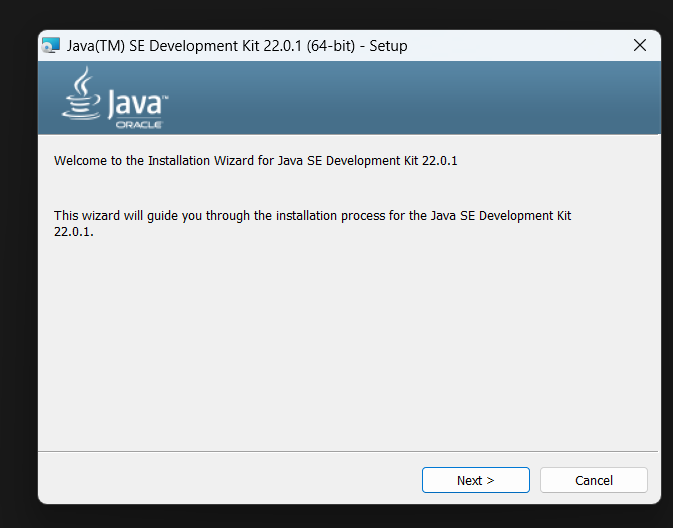
\includegraphics[width= 0.5\textwidth]{images/installazione java.png}
\end{figure}

Cliccare su \textbf{Avanti},nuovamente \textbf{Avanti} e infine, nel caso in cui l'installazione sia andata a buon fine, si dovràò cliccare sul tasto \textbf{Chiudi}.

\subsection{Variabili di ambiente}

è consigliato creare una variabile di ambiente per il JDK. Per farlo, si dovrà cercare la voce \textbf{variabili di ambiente} nella barra di ricerca di Windows e cliccare su {Modifica le variabili di ambiente per il tuo account}.

Successivamente si dovrà cliccare sul pulsante \textbf{Variabili di ambiente} e si aprirà una schermata con le variabili di ambiente. 



\begin{figure}[h!]
    \centering
    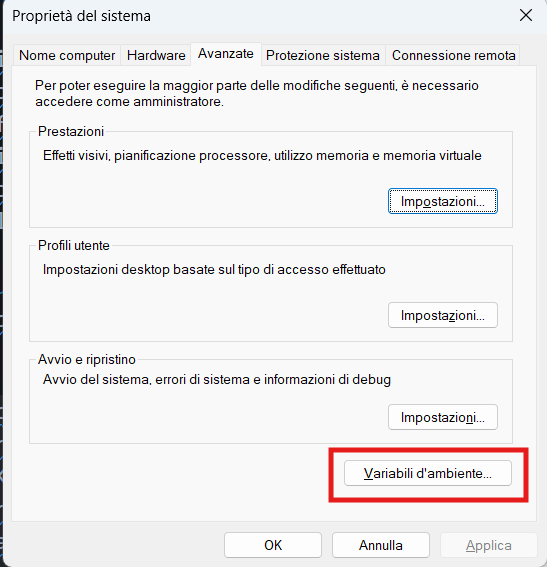
\includegraphics[width= 0.5\textwidth]{images/variabili ambienti.png}
    \caption{Schermata delle variabili di ambiente}
\end{figure}

Nella schermata, si dovra cliccare sulla variabile \texttt{PATH} e modificarla in modo da aggiungere il percorso del JDK, inserendo il percorso in cui è stato installato il JDK.

Una volta completata l'installazione del JDK, si procederà automaticamente con l'installazione del MySQL.



\subsection{Installazione MySQL}

Anche qui sarà necessario fornire i permessi di amministratore, cliccare dunque su \underline{Sì}.

\subsection{Schermata iniziale}

Dopodiché si aprirà la schermata di installazione di MySQL.

\begin{figure}[h!]
    \centering
    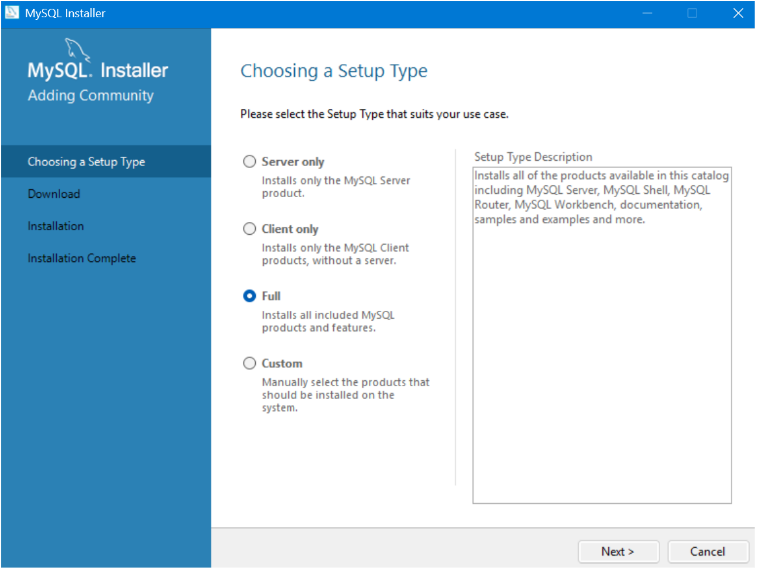
\includegraphics[width= 0.5\textwidth]{images/inizio mysql.png}
    \caption{Scelta del setup}
\end{figure}

Selezionare il tipo di setup \textbf{Full} e cliccare su \textbf{Next}. Tale scelta permetterà di installare tutti i componenti necessari per l'esecuzione del programma.

\subsection{Download dei file}

Si passerà alla schermata di download dei file necessari per l'installazione, cliccare su \textbf{Execute}. 

\begin{tcolorbox}[  colback=white!5!white, colframe=gray, title={Avvertenza} ]
    
    
    Tale schermata potrebbe richiedere un po' di tempo per il download dei file, a seconda della velocità della connessione internet. 
\end{tcolorbox}
    
Dopo aver scaricato i file, si dovrà cliccare nuovamente su \textbf{Execute}.

\begin{figure}[h!]
    \centering
    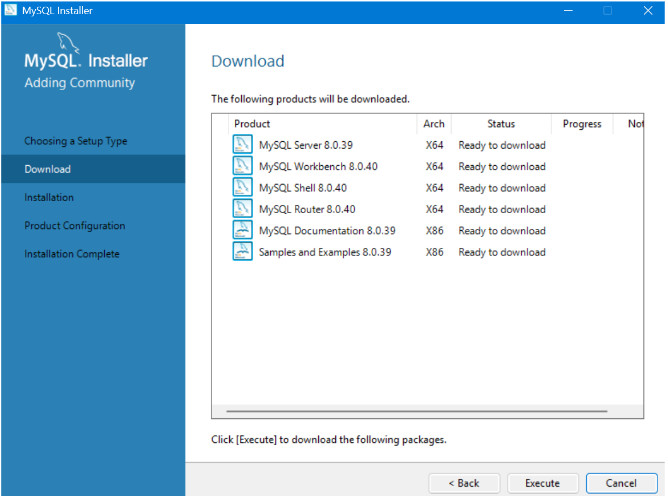
\includegraphics[width= 0.6\textwidth]{images/eexecute.png}
    \caption{Download MySQL}
\end{figure}

\subsection{Configurazione del account MySQL}
Una volta terminato il download, si procederà con la configurazione dell'account MySQL. Si dovrà quindi scegliere una password, necessaria per accedere al database. 


\begin{figure}[h!]
    \centering
    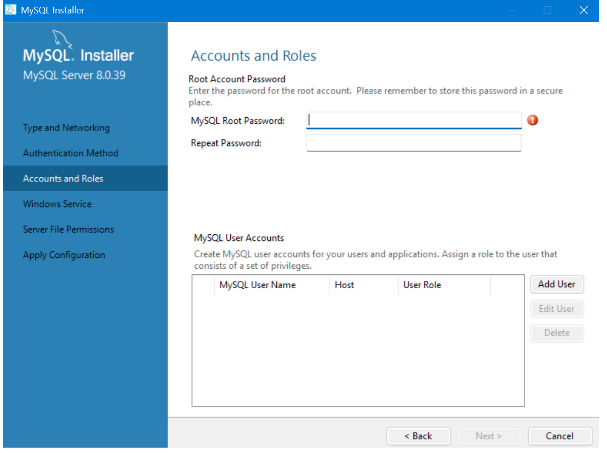
\includegraphics[width= 0.5\textwidth]{images/setup vero e proio musql.png}
    \caption{Configurazione account MySQL}
\end{figure}


Si giungerà infine alla scehermata di applicazione della configurazione del database. Cliccare su \textbf{Execute} per applicare la configurazione.

\begin{figure}[h!]
    \centering
    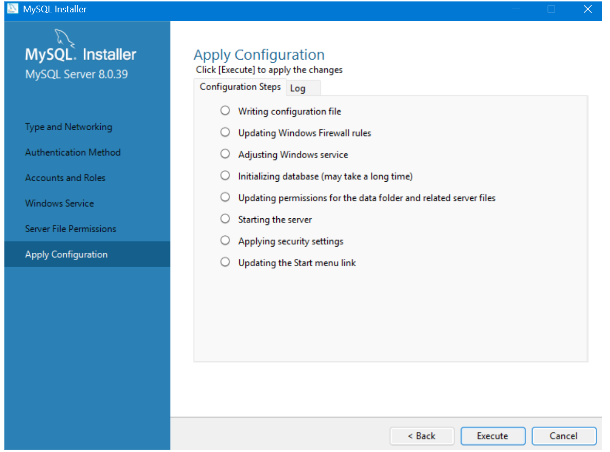
\includegraphics[width= 0.5\textwidth]{images/completamenot.png}
    \caption{Completamento installazione}
\end{figure}

Una volta terminata anche l'installazione del MySQL, si dovrà cliccare su \textbf{Finish} per chiudere l'installler. 

\begin{tcolorbox}[  colback=white!5!white, colframe=gray, title={Avvertenza} ]
    Per un corretto funzionamento sia del JDK che del MySQL, è consiglaito riavviare il computer.
    
\end{tcolorbox}


\subsection{Schermata finale}
Al termine dell'installazione il programma \texttt{resources.bat} mostrerà la seguente schermata. 

\begin{figure}[h!]
    \centering
    
\includegraphics[width= 0.6\textwidth]{images/insytllazione compeltata.png}
    \caption{Completamento installazione}
\end{figure}



\section{Eseguire il progetto base}
\subsection{Importazione del database}
Per il corretto funzionamento del progetto base, è necessario, prima di eseguire il programma, importare il database \texttt{QT.sql} presente nella cartella \texttt{Progetto\_MAP\_2/risorse/} all'interno del proprio DBMS.

Siccome nella sezione precedente abbiamo fornito l'installer per Mysql, si consiglia di utilizzare quest'ultimo per importare il database. Per importare il database all'interno di Mysql, è necessario aprire il terminale, accedere con le credenziali di root a Mysql, e lanciare il seguente comando:

\begin{verbatim}
source *PERCORSO DEL FILE QT.sql*
\end{verbatim}

\begin{tcolorbox}[  colback=white!5!white, colframe=gray, title={Avvertenza} ]

    Si ricorda di cambiare il percorso del file \texttt{QT.sql} con quello corretto, effettuando un \textit{drag and droop} del file all'interno del terminale, in modo da evitare errori di battitura. 
    
\end{tcolorbox}

Se il comando è stato eseguito correttamente, il terminale restitruirà la seguente schermata:

% \image{relazione/images/import mapdb.png}{Import del database QT}{import QT} RICORDATI DI CAMBIARE IMMAGINE IMPORT MAPDB

\subsection{Normale funzionamento}

La base dell'algoritmo permette all'utente di scegliere un raggio massimo per il cluster. 

Per ciascun punto interessato, ossia i punti con distanza inferiore al raggio impostato, l'algoritmo calcola i cluster candidati.

Una volta individuati i cluster, quello con il numero maggiore di punti verrà salvato nella cartella \texttt{./results/}, ossia nella root del progetto base. Il nome del file indicherà il database di partenza e il raggio massimo utilizzato per la ricerca, quindi scegliendo per esempio il database \texttt{gopicnic} con un raggio di 3, il file di output sarà \texttt{gopicnic\_003.dmp}.

\begin{figure}[h!]
    \centering
    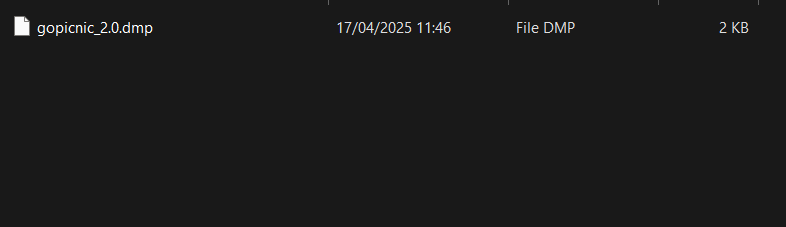
\includegraphics[width = 0.5 \textwidth]{images/results.png}
    \caption{Risultati del salvataggio}
    
\end{figure}

Una volta creato il file di output, l'algoritmo provvederà ad eliminare anche i cluster non salvati, per evitare che vengano esaminati nuovamente. 

Nel caso in cui più di un cluster abbia il numero massimo di punti, l'algoritmo ripeterà la procedura con il set ridotto di punti. 

\subsection{Struttura del progetto base}

Il progetto base consiste in un'applicazione di tipo client/server. Di fatto, nella cartella \texttt{Jar+Bat} sono presenti i file \texttt{start\_server.bat} per l'esecuzione del server e \texttt{start\_client} per il client, che non sono altro che degli script batch per l'esecuzione dei file jar.

\begin{figure}[h!]
    \centering
    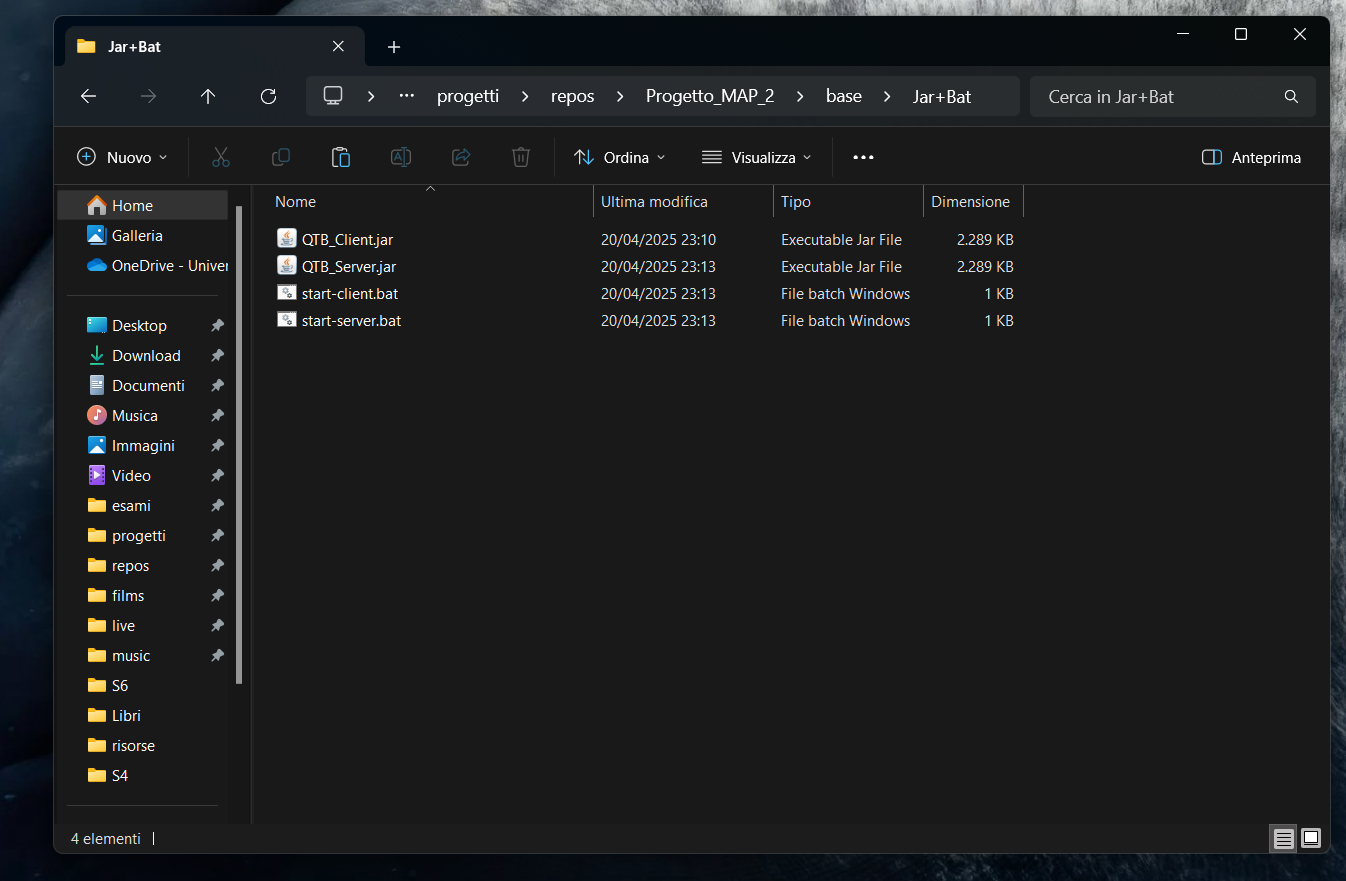
\includegraphics[width = 0.5 \textwidth]{images/file jar base.png}
    \caption{Jar del progetto base}
\end{figure}


\begin{tcolorbox}[  colback=white!5!white, colframe=gray, title={Avvertenza} ]

    Per avviare il programma correttamente, è necessario eseguire prima il file \texttt{.bat} del server e poi quello del client.
\end{tcolorbox}

\section{Avvio dell'applicazione}
\subsection{Esecuzione di QTB\_Server}

Avviando il file \texttt{start\_server.bat} verrà mostrata la seguente schermata, che indica che il server è in ascolto sulla porta 8080, in attesa di una richiesta da parte del client.

\begin{figure}[h!]
    \centering
    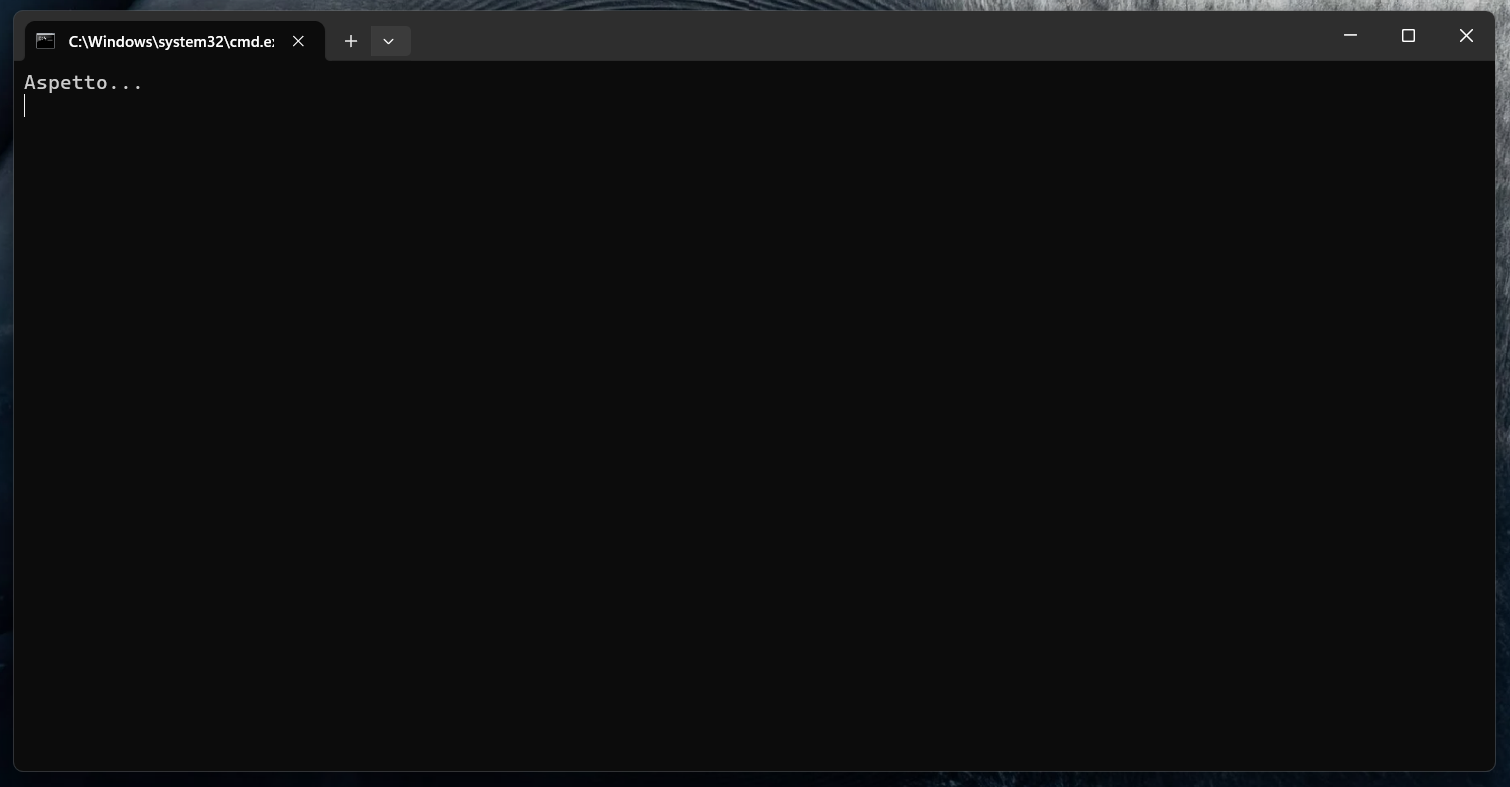
\includegraphics[width = 0.5 \textwidth]{images/normale funzionamento del server.png}
    \caption{Server in ascolto}
    
\end{figure}

\subsection{Esecuzione di QTB\_Client}

Per quanto riguarda il client, una volta avviato, mostrerà la seguente schermata.

\begin{figure}[h!]
    \centering
    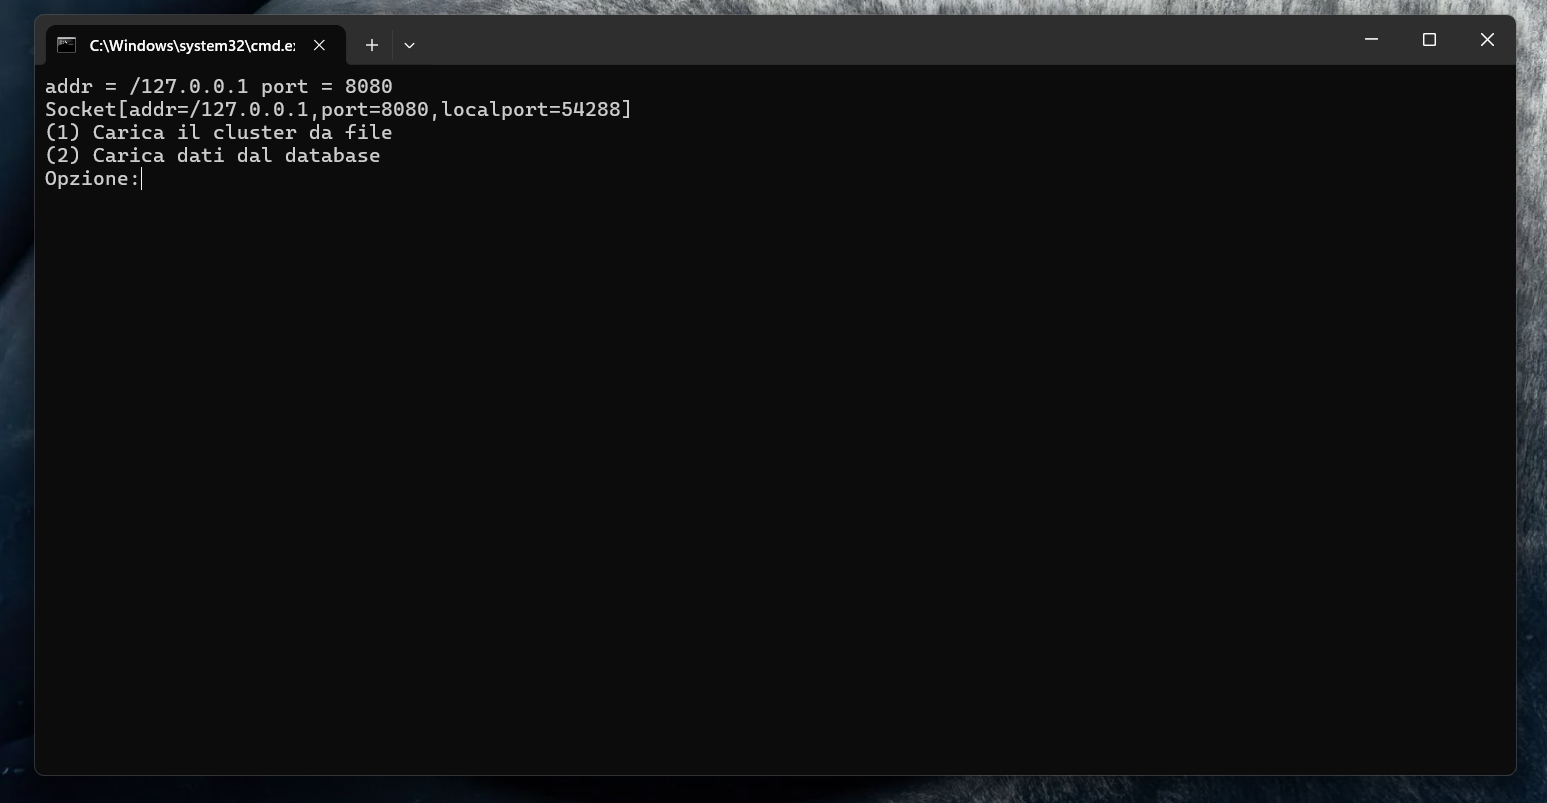
\includegraphics[width = 0.5 \textwidth]{images/normale funzionamento lcient.png}
    \caption{Schermata iniziale del client}
    
\end{figure}

\begin{tcolorbox}[  colback=white!5!white, colframe=gray, title={Avvertenza} ]

    Nel caso in cui il server non si sia avviato correttamente, o sia stato avviato il client prima del server, il client mostrerà la seguente schermata, che indicherà appunto che la connessione al server non è avvenuta correttamente.
    
    \begin{center} 
        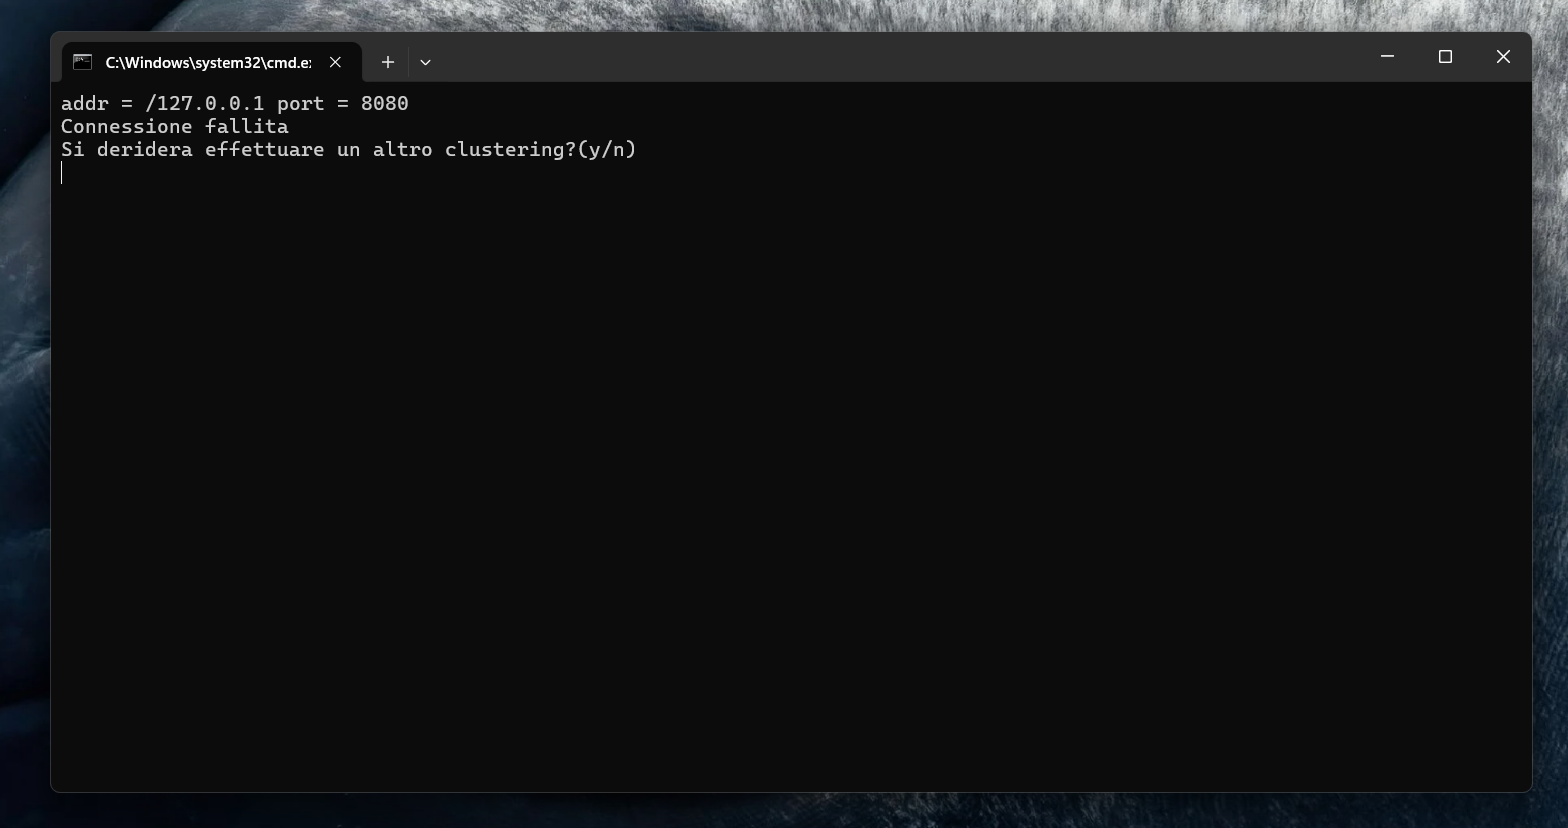
\includegraphics[width = 0.5 \textwidth]{images/connessione fallita.png}
    \end{center}
        
\end{tcolorbox}

Una volta assicurati che il client comunichi correttamente con il server, si potrà decidere se caricare i dati da un file di un clustering precedente o da un database.


Se si sceglie di caricare i dati da una tabella del database, si procederà con l'inserimento del nome della tabella da cui si vogliono estrarre i dati. Nel caso in cui tale tabella non sia presente nel database, il client avviserà l'utente con un messaggio di errore e chiedendo di inserire un nome valido. 

\begin{figure}[h!]
    \centering
    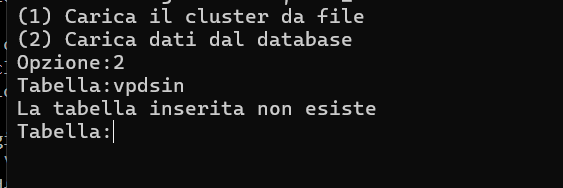
\includegraphics[width = 0.5 \textwidth]{images/teabella inesistente.png}
    \caption{Errore tabella non presente}
\end{figure}

Una volta scelto correttamente una tabella, si procederà nel determinare il raggio del clustering e, automaticamente, il programma restituirà il risultato. 

\begin{figure}[h!]
    \centering
    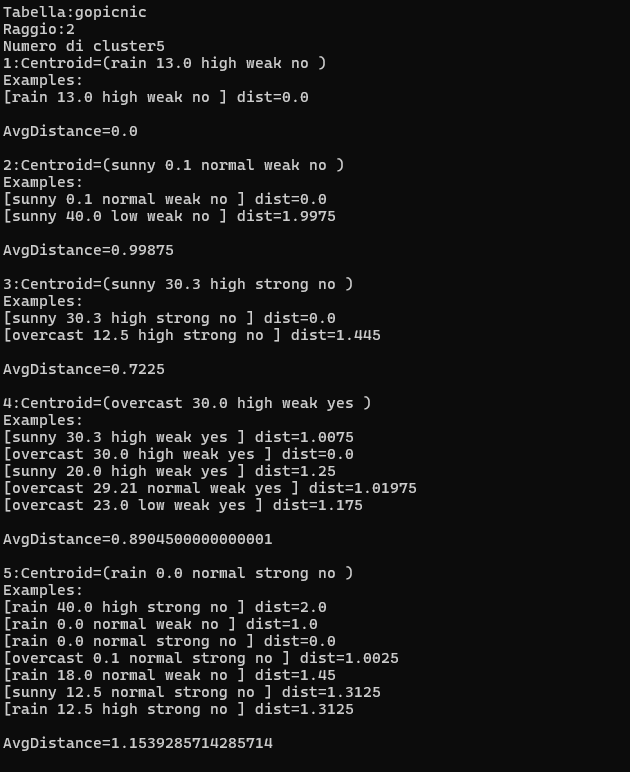
\includegraphics[width = 0.5 \textwidth]{images/risultato atteso.png}
    \caption{Risultato del clustering}
\end{figure}

A fine esecuzione, il risultato del clustering verrà salvato nella cartella \texttt{./results/} con il nome della tabella e il raggio utilizzato per il clustering, come già spiegato in precedenza.

\section{Avvio dall'ambiente di sviluppo}

È chiaramente possibile eseguire il progetto base senza passare per i file \texttt{.bat} messi a disposizione, ma direttamente da un IDE come Eclipse o IntelliJ.

In questo caso, sono necessarie alcune accortezze aggiuntive. 

\begin{tcolorbox}[  colback=white!5!white, colframe=gray, title={Avvertenza} ]

    In questa sezione si fa riferimento all'utilizzo di Visual Studio Code, ma è possibile utilizzare qualsiasi IDE che supporti Java e abbia la possibilità di eseguire file jar.

\end{tcolorbox}

Prima di tutto, occorre aprire la cartella del progetto base all'interno dell'IDE, in modo da avere un albero delle cartelle come quello mostrato in figura.

\begin{figure}[h!]
    \centering
    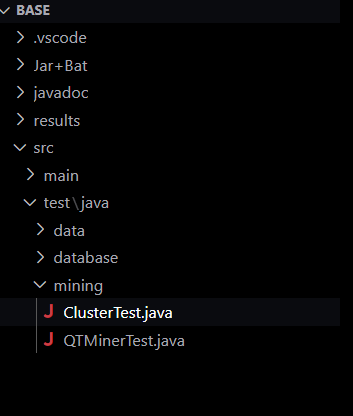
\includegraphics[width = 0.35 \textwidth]{images/albero cartelle.png}
    \caption{Sourcetree del progetto base}
\end{figure}
Una volta aspettato che Visual Studio Code abbia caricato il progetto (potrebbero volerci diversi minuti), si potrà procedere con limportazione della libreria \texttt{mysql-connector-java-8.0.32.jar} all'interno del progetto, in modo da poter utilizzare le classi necessarie per la connessione al database.

Tale libreria è presente nella cartella \texttt{Progetto\_MAP\_2/risorse/} e può essere importata all'interno del progetto in Visual Studio Code seguendo questi passaggi:

\begin{enumerate}
    \item cliccare sulla sezione \texttt{Java Projects} in basso a sinistra
    \item trovare la cartella \texttt{Referenced Libraries}
    \item cliccare con il tasto destro su \texttt{Referenced Libraries} e selezionare il tasto $+$ per aggiungere una libreria esterna
    \item selezionare il file \texttt{mysql-connector-java-8.0.32.jar} presente nella cartella \texttt{/Risorse/}
    \item attendere che Visual Studio Code abbia caricato la libreria
\end{enumerate}
\section{Test progetto base}

Durante l'esecuzione del programma, può capitare che l'utente inserisca dei valori che quest'ultimo non è in grado di gestire. Chiaramente nonostante la presenza di queste situazioni, deve essere garantita la continuità di esecuzione del programma e la corretta amministrazione di queste situazioni estreme.

\subsection{Gestione del raggio}

Nel caso in cui l'utente inserisca un valore del raggio maggiore del massimo raggio possibile, il programma restituirà un messaggio di errore e chiederà nuovamente il raggio.

Nel caso invece in cui l'utente inserisca un valore non numerico, il programma restituirà un messaggio di errore e chiederà nuovamente il raggio.

In entrambi i casi, il programma non si fermerà e continuerà a chiedere il raggio fino a quando non verrà inserito un valore corretto.

\begin{figure}[h!]
    \centering
    \subfloat[Valore del raggio troppo grande]{
        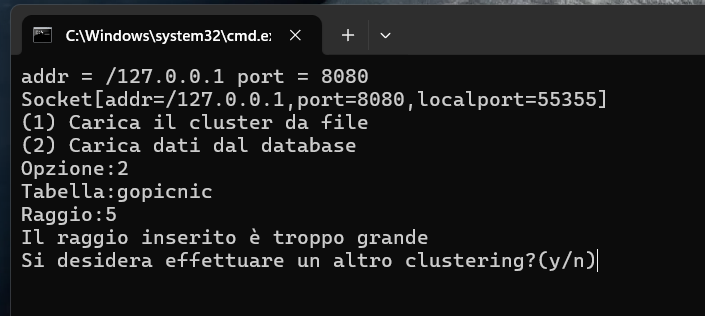
\includegraphics[width=0.45\textwidth]{images/troppo grande .png}
    }
    \hfill
    \subfloat[Valore del raggio non numerico]{
        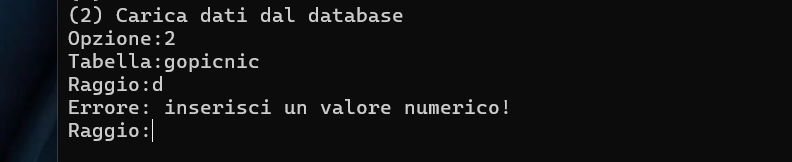
\includegraphics[width=0.45\textwidth]{images/valore non numerico .png}
    }
    \caption{Errori nel valore del raggio}
\end{figure}

\subsection{Uscita dal programma}
Una volta calcolato il raggio, il programma chiederà all'utente se ha intenzione di effettuare nuovamente un clustering: in caso positivo chiederà nuovamente la misura del raggio, in caso opposto chiederà all'utente se vuole tornare al menù principale o chiudere il programma. 


\begin{figure}[h]
    \centering
    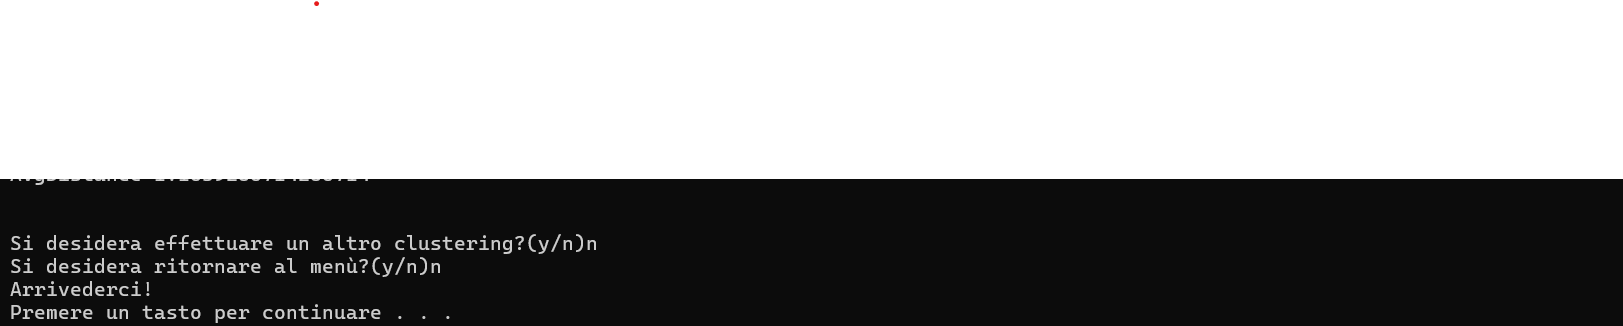
\includegraphics[width = .5\textwidth]{images/richeista continuazione.png}
    \caption{Gestione finale clustering}
\end{figure}

Domandando all'utente se si vuole ritornare al menù principale, si gestisce la chiusura del programma e, allo stesso tempo, il ritorno al menù principale, ossia alla situazione iniziale. 

Inoltre, tale stratagemma previene lo spiacevole inconveniente per cui si è obbligati a forzare l'interruzione dell'esecuzione.


\section{Eseguire il progetto esteso}

\subsection{Premessa}

Rispetto al progetto base, si è reso necessario l'utilizzo di un gestore di dipendene, in modo da poter installare le librerie necessarie per il progetto. 

\subsubsection*{Maven}

Il gestore di dipendenze scelto per questo scopo è \textbf{Maven}, il quale permette di scaricare le librerie necessarie e di gestire le versioni delle stesse.

Il vantaggio principale rispetto ad altri gestori di dipendenze, come il più blasonato Gradle, è la sua semplicità di utilizzo e la sua integrazione con gli IDE più diffusi. 

Inoltre, al contrario di Gradle, Maven non richiede la creazione di un file di configurazione complesso, ma si basa su un semplice file \texttt{pom.xml} che contiene le informazioni sulle dipendenze del progetto. 

Non richiede quindi la creazione di file di build o di scaricare i file delle dipendenze manualmente, ma il tutto viene gestito automaticamente. 

\subsubsection*{Telegram API}

Si è reso necessario l'utilizzo di un gestore delle dipendenze per via dell'utilizzo delle librerie \textbf{org.telegram.longpolling} e \textbf{org.telegram.telegrambots}, le quali permettono di interagire con l'API di Telegram. 

\subsection{Modifiche implementative}

Come accennato nella premessa, è stato implementato un bot Telegram. Tale bot permette di interagire con il progetto direttamente dall'interafccia di Telegram, rendendolo di fatto un client. 

L'adozione di Maven per la gestione delle dipendenze, inoltre ha reso inutile l'utilizzo del file \texttt{risorse.bat}, in quanto le librerie vengono scaricate automaticamente e non è più necessario gestire manualmente le versioni delle stesse.

Di per se il funzionamento del progetto non è cambiato, è stato semplicemente trasformato il modo di interazione tra esso e l'utente, trasferendola quindi da un'interfaccia cli a una più interattiva.  


\subsection{Cambiamenti rispetto versione base}



%  \section{Modifiche implementative}

Come accennato nella premessa, è stato implementato un bot Telegram. Tale bot permette di interagire con il progetto direttamente dall'interafccia di Telegram, rendendolo di fatto un client. 

L'adozione di Maven per la gestione delle dipendenze, inoltre ha reso inutile l'utilizzo del file \texttt{risorse.bat}, in quanto le librerie vengono scaricate automaticamente e non è più necessario gestire manualmente le versioni delle stesse.

Di per se il funzionamento del progetto non è cambiato, è stato semplicemente trasformato il modo di interazione tra esso e l'utente, trasferendola quindi da un'interfaccia cli a una più interattiva.  


\subsection{Cambiamenti rispetto versione base}

DAto che viene modificato solo la modalità di interazione con l'utente, la logica  di funzionamento del processo non è stata modificata rispetto alla versione base.




\section{Eseguire l'applicazione}

Rispetto alla versione base, l'usaiblità del programma è migliorata. Se prima occorreva eseguire sia il server che il client, ora è possibile eseguire un solo file JAR, che corrisponde sia al server che al modulo di comunicazione con il bot Telegram. 

\subsection{Avvio dell'applicazione}

Per avviare l'applicazione, come del resto nel progetto base, occorre spostarsi nella cartella \texttt{Jar+Bat} e eseguire il file \texttt{main.bat}. 

A differenza del progetto bas , tuttavia, all'interno della cartella in questione sarà presente solo un file \texttt{.bat}. Pertanto, sarà sufficiente eseguire tale file per avviare l'applicazione, effettuando un doppio click su di esso.

Se il file \texttt{main.bat} si apre correttamente, verrà aperta una fienstra del terminale, che mostrerà i seguenti logs: 

\image{images/avvio estensione bat.png}{Corretto avvio dell'applicazione}{avvio}

\begin{tcolorbox}[ colback=white!5!white, colframe=gray, title={Avvertenza} ]
    Si raccomanda di essere connessi ad internet, in quanto il bot Telegram necessita di una connessione per poter funzionare correttamente. Nel caso in cui si avviasse il jar del progetto esteso senza una connessione ad internet, il bot Telegram non funzionerà correttamente e non risponderà ai comandi inviati.
\end{tcolorbox}

\section{Utilizzo del bot Telegram}

Una volta avviata la comunicazione tra il server e Telegram, sarà possibile utilizzare il bot Telegram per interagire con il server.

Tale bot è raggingibile digitando il nome \texttt{@QualityTresholdBot} nella barra di ricerca di Telegram, oppure cliccando sul seguente link: \url{https://t.me/QT_Quality_Tresholdbot}

\subsection{Schermata iniziale}

Per far avviare il bot, è sufficiente premere sul pulsante \texttt{/start} presente in basso, o in alternativa, digitare il comando \texttt{/start} nella barra di testo del bot. Questo step risulta necessario per avviare la comunicazione tra il bot e il server, in modo da poter inviare e ricevere comandi.

\image{images/schermata iniziaile bot.png}{Schermata di avvio bot}{avviobot}

Una volta premuto il tasto \texttt{/start}, il bot risponderà con un messaggio di benvenuto, in cui verrà spiegato brevemente il suo scopo e l'operazione da effettuare per iniziare ad utilizzarlo.

\image{images/messaggio di benvenuto .png}{Messaggio di benvenuto del bot}{bienvenidos}
\label{Schermata iniziale}

\subsection{Comandi del bot}

Il bot Telegram implementa i seguenti comandi, nella seguente disposizione:

\begin{multicols}{2}
        \begin{itemize}
            \item \texttt{Mostra tabelle}: mostra le tabelle dei risultati ottenuti con l'algoritmo QT.
            \item \texttt{Esegui Algoritmo QT}: permette di eseguire l'algoritmo QT sui dati caricati.
            \item \texttt{Carica Risultati}: permette di caricare i risultati ottenuti dall'algoritmo QT.
            \item \texttt{Carica Risultati}: permette di caricare i risultati ottenuti dall'algoritmo QT.
            \item \texttt{Salva Risultati} : permette di salvare i risultati ottenuti dall'algoritmo QT.
            \item \texttt{Torna al menù principale} :   permette di tornare al menù principale del bot.
        \end{itemize}
\end{multicols}

\subsection{Esecuzione dell'algoritmo QT}

Chiaramente l'opzione più importante è quella che eprmette l'operazione di calcolo dell'algoritmo QT. Per eseguire l'algoritmo, è sufficiente premere il pulsante \texttt{Esegui Algoritmo QT}. 

\image{images/algoQT.png}{Opzione di esecuzione algoritmo}{eseguialgoqt}

Una volta premuto il pulsante, il bot chiederà di inserire il raggio. Tuttavia, se prima di premerlo non è stato caricata alcuna tabella proveniente dal database, il bot chiederà di caricarne una, in modo da poter eseguire l'algoritmo QT sui dati caricati.

Quindi, l'utente dovra premere il pulsante \texttt{Carica Tabella} per caricare una tabella, e successivamente premere il pulsante \texttt{Esegui Algoritmo QT} per eseguire l'algoritmo QT, specificando gli opportuni parametri richiesti.

\begin{figure}[h!]
    \centering
    \subfloat[Processo di caricamento della tabella]{
        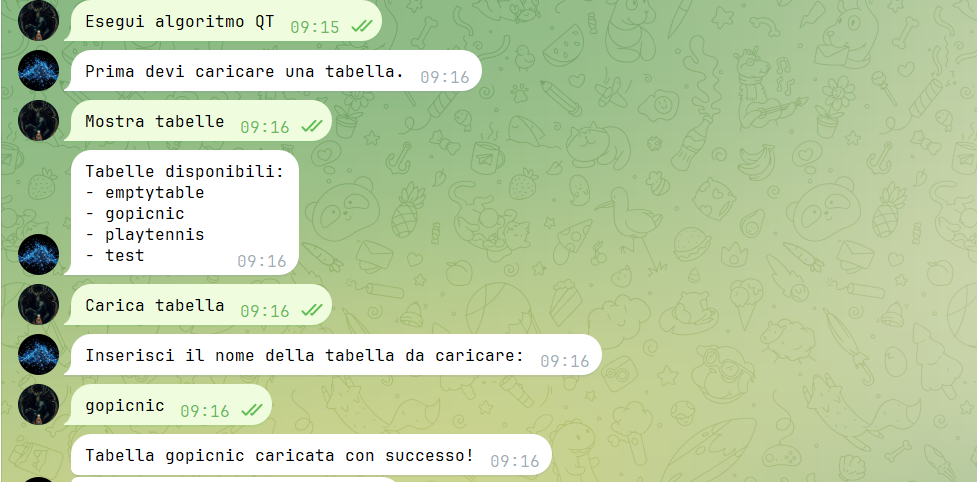
\includegraphics[width=0.45\textwidth]{images/caricamento tabella.png}
    }
    \hfill
    \subfloat[Risultato dell'esecuzione]{
        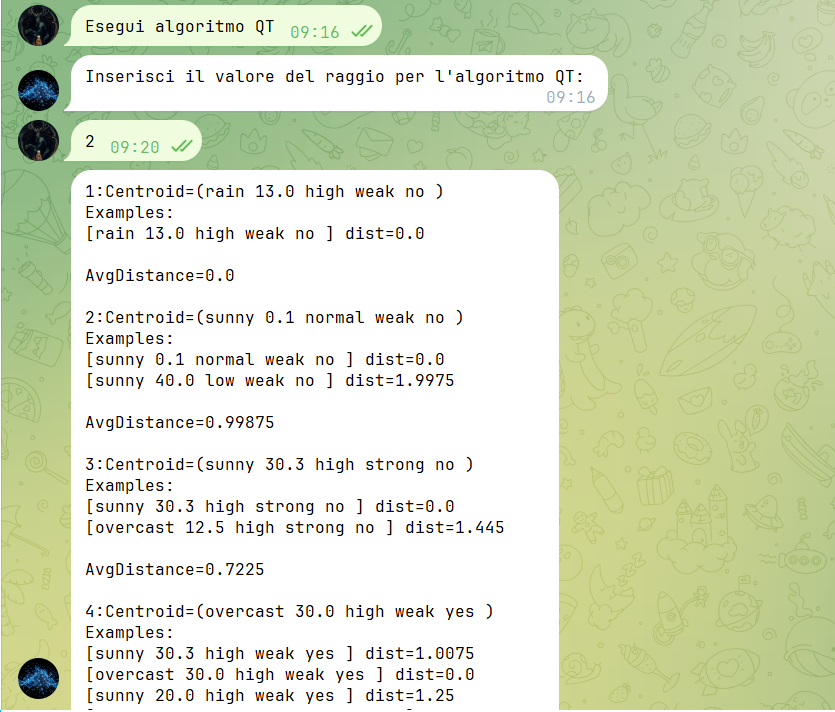
\includegraphics[width=0.45\textwidth]{images/esecuzione algoritmo.png}
    }
    \caption{Processo di esecuzione dell'algoritmo QT}
\end{figure}

\subsection{Salvare i risultati}

Una volta eseguito l'algoritmo QT, il bot permetterà di salvare il risultato dell'esecuzione in un file \texttt{.dmp}, in maniera molto simile a come avvenivna nel progetto base, all'interno della cartella \texttt{results}, presente nella cartella principale del progetto esteso. 

\image{images/cartella results.png}{Posizione cartella results}{results}

Chiaramente per eseguire tale operazione, è necessario premere il pulsante \texttt{Salva Risultati}. 

\image{images/salva risultati.png}{Opzione di salvataggio dei risultati}{salvarisultati}

\subsection{Caricare un risultato precedente}

Qualora si voglia caricare un risultato precedentemente salvato, è possibile farlo premendo il pulsante \texttt{Carica Risultati}. 

\image{images/carica risultati.png}{Opzione di caricamento dei risultati}{caricarisultati}

Il bot non chiederà direttamente di inserire il nome del file da caricare ma, dato che il nome del file \texttt{.dmp} è costruito in modo da contenere le informazioni relative al raggio e alla tabella utilizzata per l'esecuzione dell'algoritmo QT, il bot chiederà di inserire il raggio e  la tabella da ritrovare. 

Se il file \texttt{.dmp} esiste, il bot risponderà restituendo il risultato dell'esecuzione in questione. 

\image{images/risultato caaricamento .png}{Risultato del caricamento di un file .dmp}{riscaricamento}

\subsection{Ritono al menù principale}

Qualora si voglia far ripartire il bot dalla schermata iniziale, è possibile farlo premendo il pulsante \texttt{Torna al menù principale}.

Una volta premuto il pulsante, il bot risponderà con un messaggio di benvenuto, come quello mostrato alla fine della sezione \ref{Schermata iniziale}.


\section{Test progetto esteso}

Durante la fase di test del progetto esteso, sono stati eseguiti diversi test per verificare il corretto funzionamento delle varie funzionalità dei comandi implmentanti. 
Tali test hanno coinvolto principalmente la correttezza della gestione delle varie situaioni anomale che possono incorrere durante l'esecuzione dei comandi, come ad esempio la gestione di file non trovati, errori di sintassi o problemi di accesso ai file.

Chiaramente queste situazioni anomale devono essere notificate al livello di client, per permettere all'utente di comprendere l'entità del problema e prendere le opportune misure.

Si fa notare che i test elencati sono stati eseguiti tenendo conto il normale flusso di lavoro del bot, nel senso che è stato seguito il flusso di interazione del bot per via sequenziale, senza saltare passaggi o inviare comandi in modo casuale.

\subsection{Tabelle non trovate}

Nel caso in cui venga inserito il nome di una tabella inesistente, il bot risponderà specificando che  la tabella isnerita non esiste e invita a inserire un nome di tabella valido.

\image{images/tabella inesistente.png}{comportamento tabella inesistente}{tabne}

Chiaramente l'algoritmo QT non potrà essere eseguito su una tabella inesistente, quindi il bot risponderà con un messaggio di errore specificando che non è possibile eseguire l'algoritmo QT se prima non viene caricata una tabella valida.

\image{images/esegui prima qt.png}{inconsistenza algoritmo QT}{inconsistenza}

\subsection{raggio non valido}

Nel caso si inserisca un raggio non valido, che include quindi le casistiche in cui il raggio è negativo o non numerico, il bot risponderà specificando che il raggio inserito non è valido, in quanto genererebbe un solo cluster, e pertanto  invita a inserire un raggio valido.

\image{images/raggio invalido.png}{Raggio invalido}{raggoinv}

\subsection{File non trovato}

Nel caso in cui, durante l'esecuzione del comando \texttt{Carica risultati}, il file specificato non dovesse essere presente enlla cartella \texttt{results}, il bot risponderà specificando che il file non è stato trovato. 

\image{images/file not found.png}{Esempio di file non trovato}{fnf}

Sarà quindi necessario eseguire nuovamente il comando ed inserire il nome di un file valido. 

\end{document}